\documentclass[../SpecificaTecnica.tex]{subfiles}
\begin{document}
\section{Descrizione design pattern}
	\subsection{Design pattern architetturali}
		\subsubsection{MVP}
		
		\begin{figure}[!h]
		\centering
		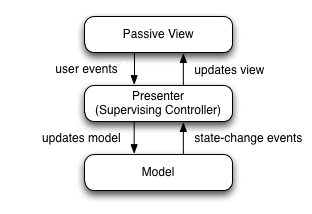
\includegraphics[scale=0.6]{pattern/mvp}
			\caption{Struttura del pattern MVP}
		\label{fig:Struttura_MVP}
	\end{figure}
	
			Model-View-Presenter (MVP) è un pattern architetturale derivato dal MVC (Model-View-Controller), utilizzato per dividere il codice in funzionalità distinte. Il suo principale ambito di utilizzo è nelle applicazioni un insieme di informazioni deve essere rappresentato mediante un'interfaccia grafica.
			\paragraph{Componenti}
			MVC è basato sul principio di disaccoppiamento di tre oggetti distinti, riducendo in questo modo le dipendenze reciproche; inoltre permette di fornire una maggiore modularità, manutenibilità e robustezza al software.
				\subparagraph{Model}
					Il Model rappresenta il cuore dell'applicazione: esso definisce il modello dei dati definendo gli oggetti secondo la logica di utilizzo dell'applicazione, ossia la sua business logic. Inoltre, indica le possibili operazioni che si possono effettuare sui dati.
				\subparagraph{View}
					Nel pattern MVP, il Model è un componente prevalentemente passivo, ma si occupa anche di notificare al Presenter eventuali modifiche del proprio stato. Nella struttura del pattern MVP, la View si occupa di prendere gli input dell'utente e passarli al Controller, affinché esegua operazioni sul Model.
				\subparagraph{Presenter}
					Il Presenter è l'intermediario tra il Model e la View. Si occupa di implementare l'insieme di operazioni eseguibili sul modello dei dati attraverso una particolare vista, ossia l'application logic. Ad ogni View, deve corrispondere un diverso Controller.
				\paragraph{Vantaggi}
					Elenco vantaggi.
				\paragraph{Svantaggi}
					Elenco svantaggi.
			\subsubsection{Dependency injection}
			
				\paragraph{Vantaggi}
					Elenco vantaggi.
				\paragraph{Svantaggi}
					Elenco svantaggi.
	\subsection{Design pattern creazionali}
		\subsubsection{Singleton}
		
			\paragraph{Vantaggi}
				Elenco vantaggi.
			\paragraph{Svantaggi}
				Elenco svantaggi.
		\subsubsection{Strategy}
		
			\paragraph{Vantaggi}
				Elenco vantaggi.
			\paragraph{Svantaggi}
				Elenco svantaggi.
	\subsection{Design pattern strutturali}
		\subsubsection{Facade}
		
			\paragraph{Vantaggi}
				Elenco vantaggi.
			\paragraph{Svantaggi}
				Elenco svantaggi.
	\subsection{Design pattern comportamentali}
		\subsubsection{Observer}
		
			\paragraph{Vantaggi}
				Elenco vantaggi.
			\paragraph{Svantaggi}
				Elenco svantaggi.
\end{document}